% Needs 2 passes, as the overlay is used!
\documentclass[margin=2pt]{standalone}
\usepackage[table]{xcolor}
\usepackage[utf8]{inputenc}
\usepackage[T1]{fontenc}

\usepackage{tikz}
\usepackage{helvet}
\usepackage{amsmath}
\usepackage{array}
\usepackage{tabularray}

\renewcommand\familydefault\sfdefault
\newcommand{\DisplayDirectory}{1}
\newcommand{\DisplayArrows}{1}

\usetikzlibrary{intersections, shapes.arrows, spath3, shapes.geometric, fit, backgrounds, calc, tikzmark}

\definecolor{themeBlue}{RGB}{1, 103, 143}
\definecolor{themeOrange}{RGB}{221, 109, 16}
\definecolor{themeTeal}{RGB}{18, 54, 69}
\definecolor{themeGrey}{RGB}{120, 121, 124}

\begin{document}
    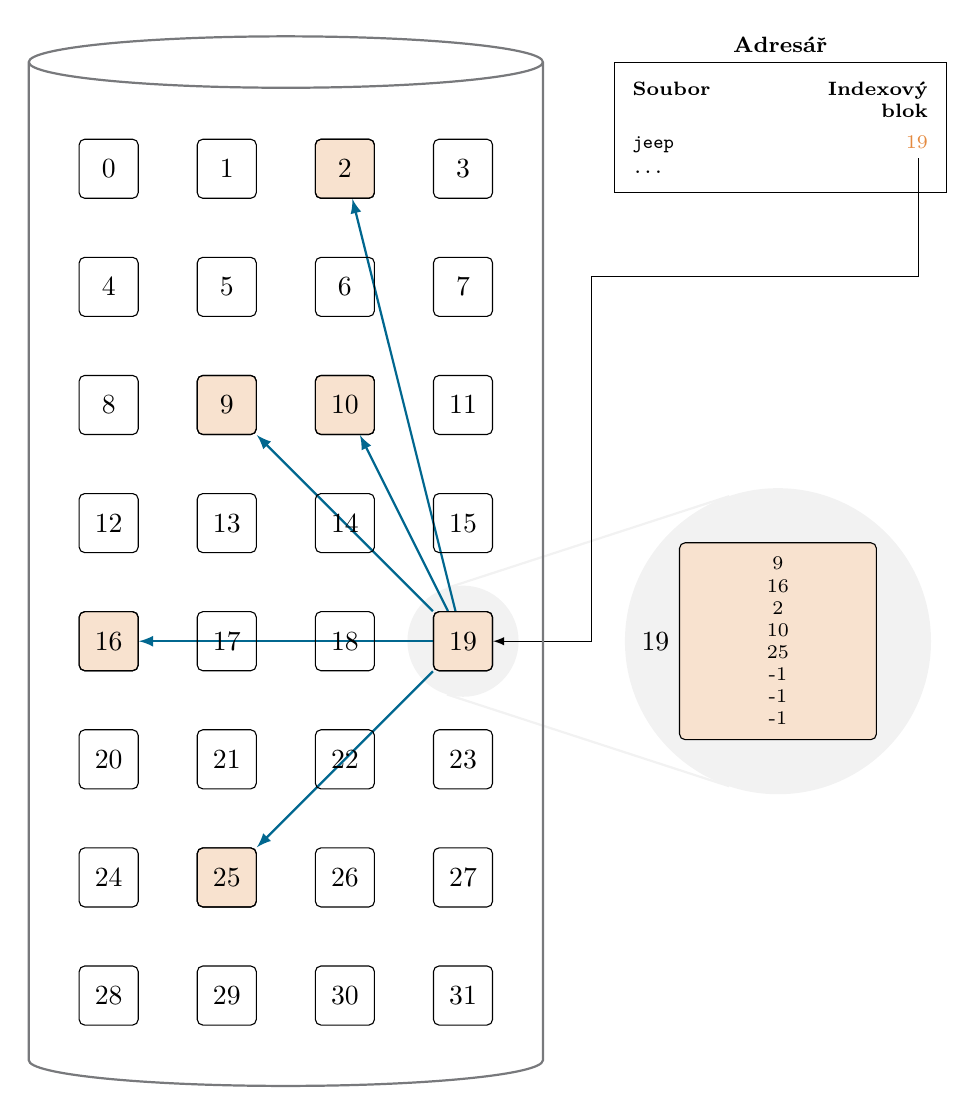
\begin{tikzpicture} [
        bus/.style={single arrow, single arrow head extend=2pt},
        hdd/.style={thick, cylinder, inner sep = 18pt, shape border rotate = 90, draw = themeGrey, aspect=0.1},
        cluster/.style={draw, minimum size=0.75cm, rounded corners=2pt},
        l/.style={align=left},
        r/.style={align=right},
        c/.style={align=center}
    ]
        \foreach \y in {0, ..., 7} {
            \foreach \x in {0, ..., 3} {
                \pgfmathtruncatemacro{\label}{\x + (\y * 4)}
               \node [cluster]  (\label) at (1.5*\x, -1.5*\y) {\label}; 
            }
        }
        \draw node[hdd, fit=(0) (31)] (c) {};

        \ifnum\DisplayDirectory=1
            \draw (19) ++(4,0) node[cluster, fill=themeOrange!20, minimum size=2.5cm, c, font=\scriptsize] (inode) {
                    9\\
                    16\\
                    2\\
                    10\\
                    25\\
                    -1\\
                    -1\\
                    -1
                };
            \draw (inode.west) node[left] {19};
        \fi
        
        \begin{scope}[on background layer]
            \ifnum\DisplayDirectory=1
                \draw node[fill=themeGrey!10, circle, fit=(inode), outer sep=0] (zoom) {};
                \draw node[fill=themeGrey!10, circle, fit=(19), outer sep=0] (direct) {};
    
                \draw[thick, themeGrey!10] 
                    (tangent cs:node=direct,point={(zoom.south)},solution=2) 
                    -- (tangent cs:node=zoom,point={(direct.south)});
                \draw[thick, themeGrey!10] 
                    (tangent cs:node=direct,point={(zoom.north)},solution=1) 
                    -- (tangent cs:node=zoom,point={(direct.north)},solution=2);
            \fi
            
            \draw (19) node [cluster, fill=themeOrange!20] {};
            \foreach \n in {2, 9, 10, 16, 25} {
                \draw (\n) node [cluster, fill=themeOrange!20] {};
                \ifnum\DisplayArrows=1
                    \draw[-latex, draw=themeBlue, thick] (19) -- (\n);
                \fi
            }
            \ifnum\DisplayDirectory=1
                \draw[latex-] (19.east) -- ++(1.25, 0) coordinate (fs_in);
            \fi
        \end{scope}
    
        \ifnum\DisplayDirectory=1
            \matrix (table) [draw, text width=5em, font=\scriptsize, anchor=north] at ($ (c.north east|-c.after top) +(3, 0) $) {
                \node[l] {\textbf{Soubor}};     & \node[r] {\textbf{Indexový blok}}; \\
                \node[l] {\texttt{jeep}};     & \node[r] (f19) { \textcolor{themeOrange!80}{19} };      \\
                \node[l] {\texttt{\dots}};      & \node[r] { };        \\
            };
            \draw (table.north) node[above, anchor=south, font=\footnotesize] {\textbf{Adresář}};

             \draw (f19.south east) ++(-7pt, 0pt) to ++(0, -1.5) to (fs_in|-\tikztostart) to (fs_in);
        \fi
    \end{tikzpicture}
\end{document}